\section{Results}
\label{sec:results}

\begin{table}[t]
\caption{Pre-registered hypotheses ($n$ programs; one-sided Wilcoxon, Holm across the four).}
\label{tab:primary}
\small
\begin{tabular}{@{}lllll@{}}
\toprule
 & Effect & $n$ & Holm $p$ & Supported \\
\midrule
H1 headroom & ratio \HOneRatio{} [\HOneLo, \HOneHi] & \HOnePrograms & $\HOnePHolm$ & yes \\
H2 drift & median $\rho$ \HTwoRho{} [\HTwoLo, \HTwoHi] & \HTwoPrograms & $\HTwoPHolm$ & yes \\
H3 predictable & residual $R^2$ \HThreeRsq & \HThreePrograms & $\HThreePHolm$ & yes \\
H4 re-prediction & ratio \HFourRatio{} [\HFourLo, \HFourHi] & \HFourPrograms & $\HFourPHolm$ & \textbf{no} \\
\bottomrule
\end{tabular}
\end{table}

Table~\ref{tab:primary} summarises the four pre-registered tests. Three are supported and one is
not.

\subsection{H1: Program-specific headroom}
With the same beam builder and a budget of ten evaluations, ordering with the program's own graph
gives a geomean IR instruction count \HOneRatio{} times that of the static graph (95\% CI
\HOneLo--\HOneHi). It is better on \HOneWins{} programs and worse on \HOneLosses{}. The oracle graph
is not a usable method: it costs \NPairs{} extra measurements. H1 measures how much a static graph
leaves on the table.

\emph{Exploratory: does the headroom reach machine code?} It does for code size on both targets.
The oracle-graph sequences are \MSizeXPct\% smaller in x86-64 \texttt{.text} (ratio \MSizeXRatio,
CI \MSizeXLo--\MSizeXHi, $p=\MSizeXP$) and \MSizeAPct\% smaller on AArch64 (\MSizeARatio,
$p=\MSizeAP$; \MSizeATwoHundredRatio{} at $\E=200$). For executed instructions (\MDynRatio, CI
\MDynLo--\MDynHi) and wall-clock time (\MRuntimeRatio, CI \MRuntimeLo--\MRuntimeHi,
\MRuntimePrograms{} programs) the direction is the same, but the intervals include or touch 1, so
we call this suggestive only.

\emph{Exploratory: where the variance lies.} In a variance decomposition of $I$ over pair, program
and snapshot, the pair alone explains \VdPair\% of the variance. Terms involving the program
explain \VdProg\% (bootstrap CI over programs \VdProgLo--\VdProgHi\%). A static graph captures only
the pair term. Built LOPO, its interactions correlate with a program's own at S0 with median
Spearman \SgeRhoSZero.

\subsection{H2: Interactions drift during optimization}
Over pairs that are non-weak at S0 or S2, the median per-program Spearman correlation between a
program's S0 and S2 interactions is \HTwoRho{} (CI \HTwoLo--\HTwoHi; \HTwoPrograms{} programs with
enough non-weak pairs), well below the pre-registered 0.5.

\emph{Exploratory: where the drift happens.} Figure~\ref{fig:drift} shows all snapshot pairs. The
correlation with raw IR falls to \RhoZeroOne{} after early simplification alone and stays near that
level (\RhoZeroTwo, \RhoZeroThree, \RhoZeroFour). Later snapshots resemble each other more:
\RhoOneTwo{} between S1 and S2, \RhoTwoThree{} between S2 and S3, and \RhoTwoFour{} between S2 and
S4. Interactions are also sparse: \SparseZero\% of pairs are weak at S0, rising to \SparseFour\% at
S4. A graph measured on raw IR therefore describes the IR that later passes see poorly.

\begin{figure}[t]
\centering
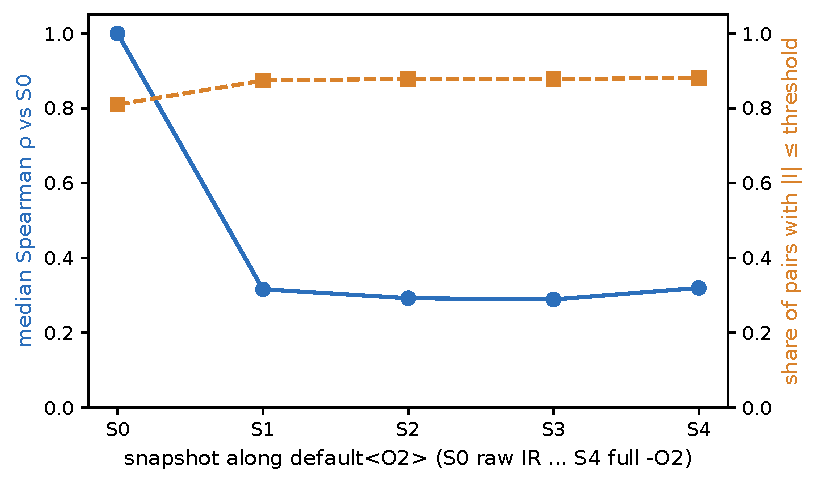
\includegraphics[width=0.49\columnwidth]{figures/v3_1_drift_decay.pdf}\hfill
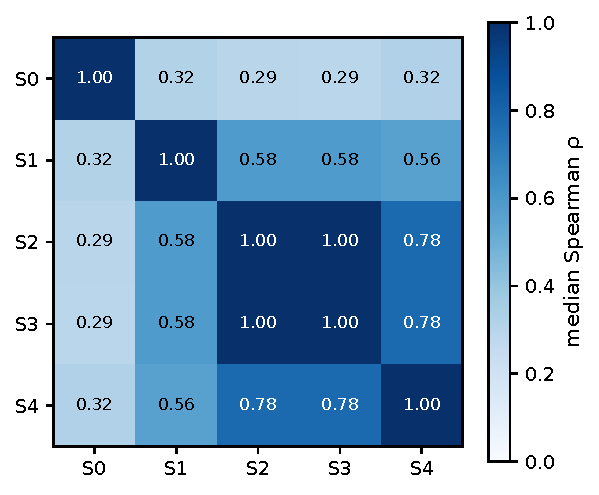
\includegraphics[width=0.47\columnwidth]{figures/v3_1_drift_matrix.pdf}
\caption{Drift along LLVM's \Otwo{} pipeline (exploratory). Left: median per-program Spearman
$\rho$ with S0 and the share of weak pairs. Right: median $\rho$ between every pair of snapshots.}
\label{fig:drift}
\end{figure}

\subsection{H3: Per-program interactions are predictable}
The LOPO model's mean absolute error is \HThreeMaeModel{}, against \HThreeMaeStatic{} for the static
graph. It removes \HThreeGap\% of the static graph's error (residual $R^2 = \HThreeRsq$) and is
better on \HThreeBetter{} of \HThreePrograms{} held-out programs (worse on \HThreeWorse).
Exploratory: for single-pass gains, the quantity re-prediction uses, the model ranks passes better
than the static graph at every snapshot (median Spearman \RankModelSZero{} vs.\ \RankStaticSZero{} at
S0, and \RankModelSTwo{} vs.\ \RankStaticSTwo{} at S2).

\subsection{H4: Re-prediction does not win at ten compilations}
The strongest other method at $\E=10$, chosen by the pre-registered rule, was the GA (\texttt{\HFourOther}). Re-prediction's IR count is \HFourRatio{} times
the GA's (\HFourWorse\% worse; better on \HFourWins{} programs, worse on \HFourLosses{}; Holm
$p=\HFourPHolm$). H4 is not supported. Figure~\ref{fig:curves} shows all methods across budgets.

\begin{figure}[t]
\centering
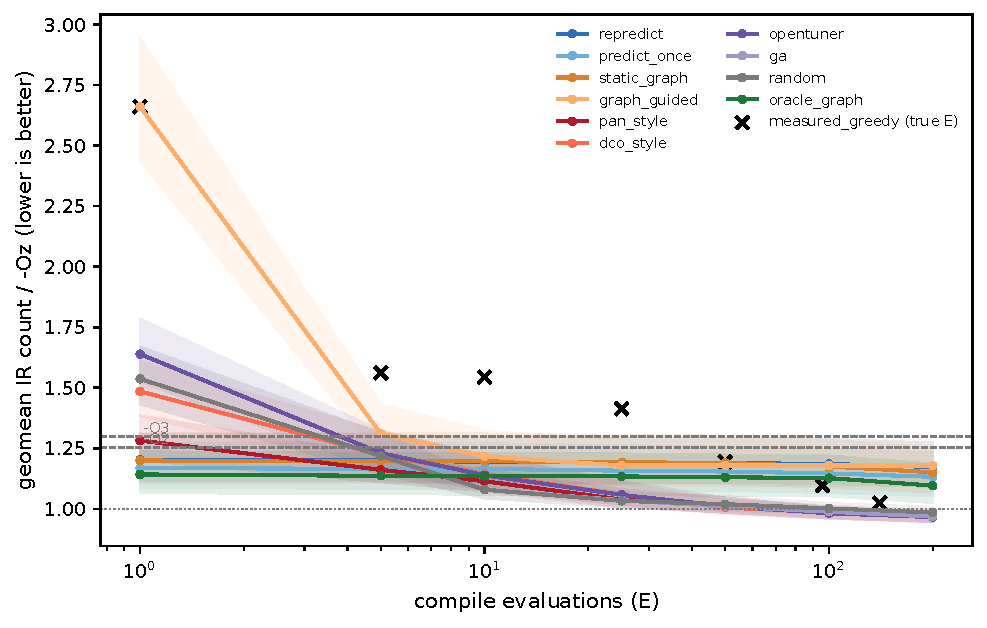
\includegraphics[width=\columnwidth]{figures/v3_1_budget_curves.pdf}
\caption{Best-so-far IR instruction count relative to \Oz{} (geomean over programs; lower is better)
by compile budget \E.}
\label{fig:curves}
\end{figure}

\subsection{Exploratory: why re-prediction loses}
The predictions are not the weak part (H3). The bottleneck is turning a graph into sequences.
\begin{itemize}
\item \textbf{Graph builders plateau.} From $\E=1$ to $\E=200$ the median per-program improvement is
\PlateauRepredict\% for re-prediction, \PlateauPredOnce\% for predict-once, \PlateauOracle\% for the
oracle graph and \PlateauStatic\% for the static graph. The GA improves by \PlateauGA\% and OpenTuner
by \PlateauOpenTuner\%. A pairwise additive estimate ranks a narrow family of similar sequences, and
spending more budget only walks down that family.
\item \textbf{Even perfect pair information does not beat search at $\E=10$.} The oracle graph's
ratio to the GA is \XOracleGARatio{} (CI \XOracleGALo--\XOracleGAHi, $p=\XOracleGAP$).
\item \textbf{Re-conditioning adds nothing under this builder.} Re-prediction vs.\ the static graph
gives \XRepStaticRatio{} ($p=\XRepStaticP$). Against predict-once it gives \XRepOnceRatio.
\item \textbf{At one compilation, predicted graphs win.} At $\E=1$ the strongest search method is
Pan-style. Predict-once beats it on \XOnceEOneWins{} of \XOnceEOnePrograms{} programs (ratio
\XOnceEOneRatio, CI \XOnceEOneLo--\XOnceEOneHi, $p=\XOnceEOneP$). Re-prediction gives
\XRepEOneRatio{} ($p=\XRepEOneP$) and the oracle graph \XOracleEOneRatio. By $\E=5$ the advantage is
gone (predict-once vs.\ Pan-style: \XOnceEFiveRatio).
\end{itemize}
